\documentclass[border=10pt,convert]{standalone}
\usepackage{tikz}
\usetikzlibrary{positioning,shapes.multipart,shapes}
\begin{document}
\newcommand { \key }[1]{\underline{#1}}
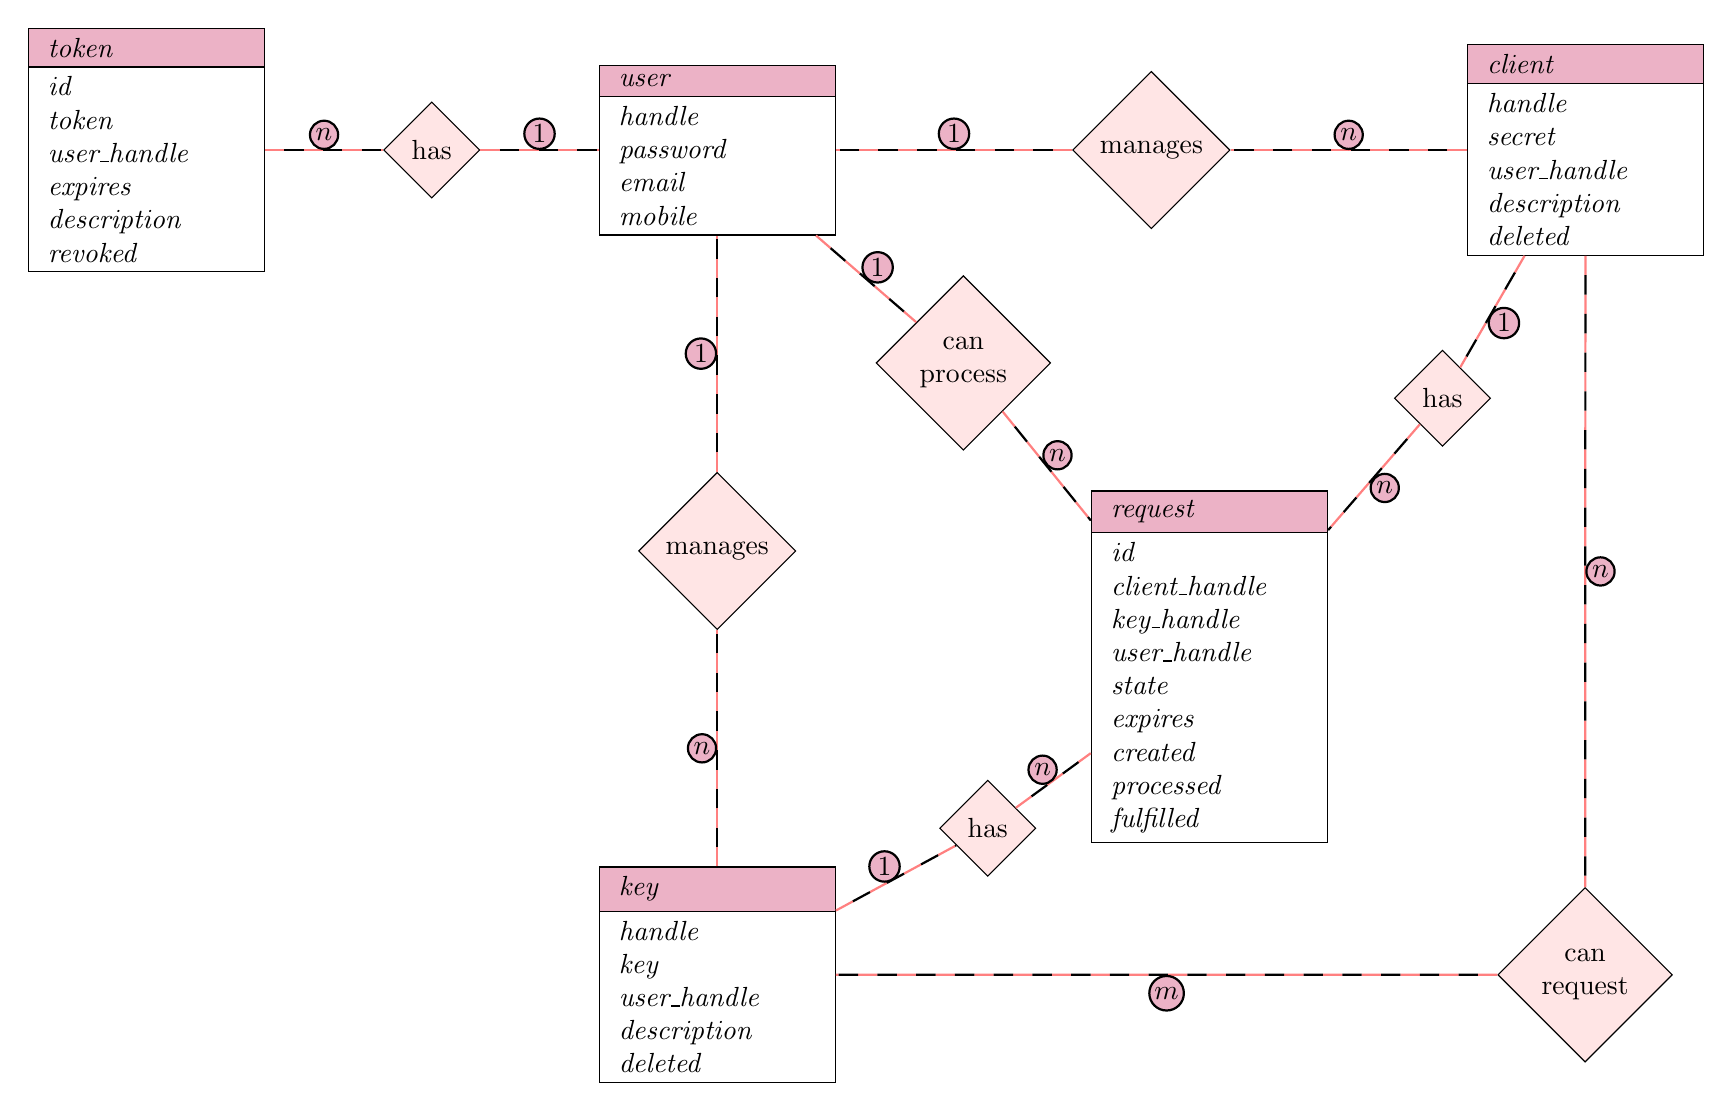
\begin{tikzpicture}[
    auto,
    node distance=1.5cm,
    basic/.style={
      align=left,
      draw,
      font=\itshape,
      rectangle split,
      rectangle split parts=2,
      rectangle split part fill={purple!30,white},
      minimum width=3cm,
      text width=2.5cm,
    },
    double dashed/.style={
      dashed,
      dash pattern = on 7pt off 7pt,
      thick,
      red!50,
      postaction={
          black,
          dash phase = 7pt,
          draw,
      }
    },
    quantity/.style={
      black,
      circle,
      draw,
      fill = purple!30,
      inner sep = 1pt,
      solid,
    },
    relation/.style={
      align=center,
      diamond,
      draw,
      fill = red!10,
      text centered,
    }]
  \node[basic] (user) {user
    \nodepart{second}
    \key{handle}\\
    password\\
    email\\
    mobile
  };
  \node[relation, right = 3 of user] (rel_client_user) {manages};
  \node[relation, below = 3 of user] (rel_key_user) {manages};
  \node[relation, below right = of user] (rel_request_user) {can\\process};
  \node[relation, left = of user] (rel_token_user) {has};

  \node[basic, left = of rel_token_user] (token) {token
    \nodepart{second}
    \key{id}\\
    token\\
    user\_handle\\
    expires\\
    description\\
    revoked
  };

  \node[basic, right = 3 of rel_client_user] (client) {client
    \nodepart{second}
    \key{handle}\\
    secret\\
    user\_handle\\
    description\\
    deleted
  };

  \node[basic, below right = of rel_request_user] (request) {request
    \nodepart{second}
    \key{id}\\
    client\_handle\\
    key\_handle\\
    user\_handle\\
    state\\
    expires\\
    created\\
    processed\\
    fulfilled
  };

  \node[basic, below = 3 of rel_key_user] (key) {key
    \nodepart{second}
    \key{handle}\\
    key\\
    user\_handle\\
    description\\
    deleted
  };
  \node[relation, below left = 1.5 and 0 of client] (rel_client_request) {has};
  \node[relation, below left = -0.5 and 1 of request] (rel_key_request) {has};
  \node[relation, right = 8.4 of key] (rel_client_key) {can\\request};

  \draw[double dashed] (client) -- (rel_client_user) node[above,midway,quantity] {\(n\)} -- (user) node[above,midway,quantity] {1};
  \draw[double dashed] (key) -- (rel_key_user) node[midway,quantity] {\(n\)} -- (user) node[midway,quantity] {1};
  \draw[double dashed] (token) -- (rel_token_user) node[midway,quantity] {\(n\)} -- (user) node[midway,quantity] {1};
  \draw[double dashed] (user) -- (rel_request_user) node[midway,quantity] {1} -- (request) node[midway,quantity] {\(n\)};
  \draw[double dashed] (client) -- (rel_client_key) node[midway,quantity] {\(n\)} -- (key) node[midway,quantity] {\(m\)};
  \draw[double dashed] (client) -- (rel_client_request) node[midway,quantity] {1} -- (request) node[midway,quantity] {\(n\)};
  \draw[double dashed] (key) -- (rel_key_request) node[midway,quantity] {1} -- (request) node[midway,quantity] {\(n\)};
\end{tikzpicture}
\end{document}